\subsection{Speed autopilot}\label{subsec:prob1.2}
To control the surge speed of MS Fartøystyring we suggest using a linearized model, where the surge speed is decoupled from the rest of the system. We are assuming $$u>>v$$ which leads to $$U=u$$.
We then use a quadratic speed model
\begin{equation}
K_1 \dot{u} - X_u u_r - X_{|u| u} |u_r| u_r=\tau
\end{equation}
which leads to
\begin{equation}
\dot{u} = \frac{ \tau + X_{|u|u} |u_r| u_r +X_u u_r }{ m-X_{\dot{u}} } 
= \frac{X_{|u|u} |u_r| u_r +X_u u_r }{ m-X_{\dot{u}} } + \tau_{nl}
\end{equation}
where
\begin{equation}
\tau_{nl}  = \frac{ \tau}{ m-X_{\dot{u}} } \Rightarrow \tau = \tau_{nl}(m-X_{\dot{u}})
\end{equation}

\begin{figure}[H]
    \centering
    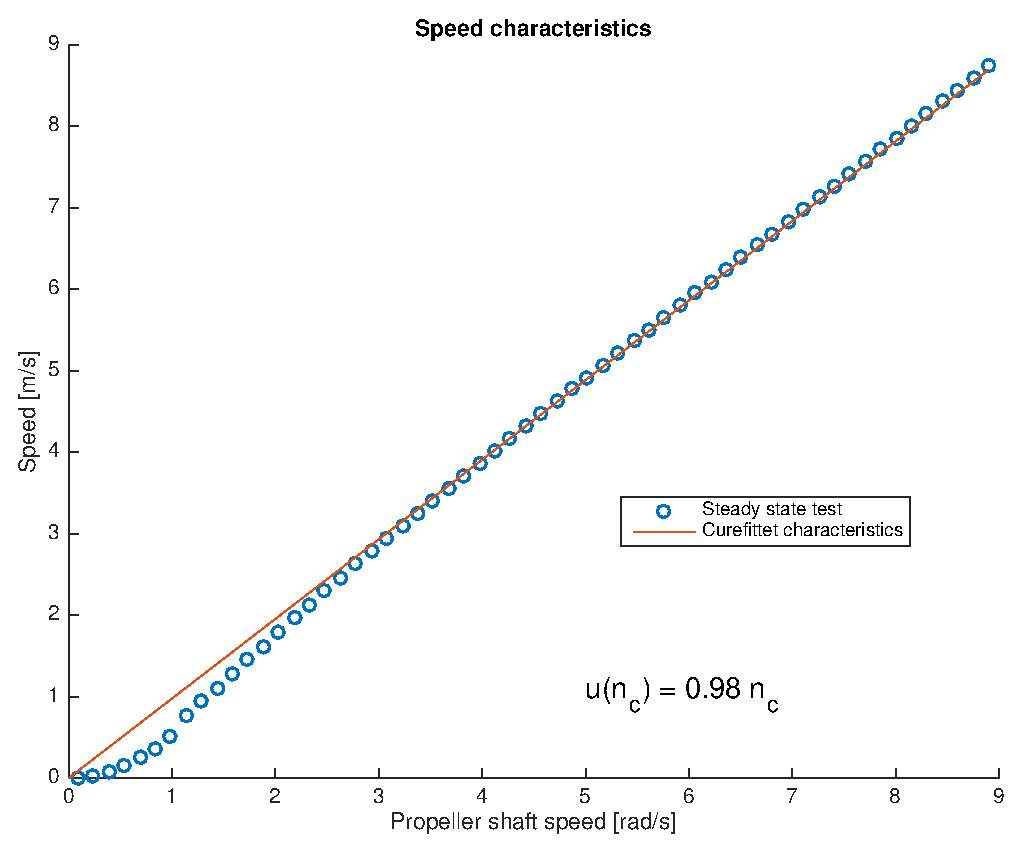
\includegraphics[width=0.9 \textwidth]{task1.8/Speed_characteristics}
    \caption{Speed characteristics}
    \label{fig:1.8-speed}
\end{figure}

\begin{figure}[H]
    \centering
    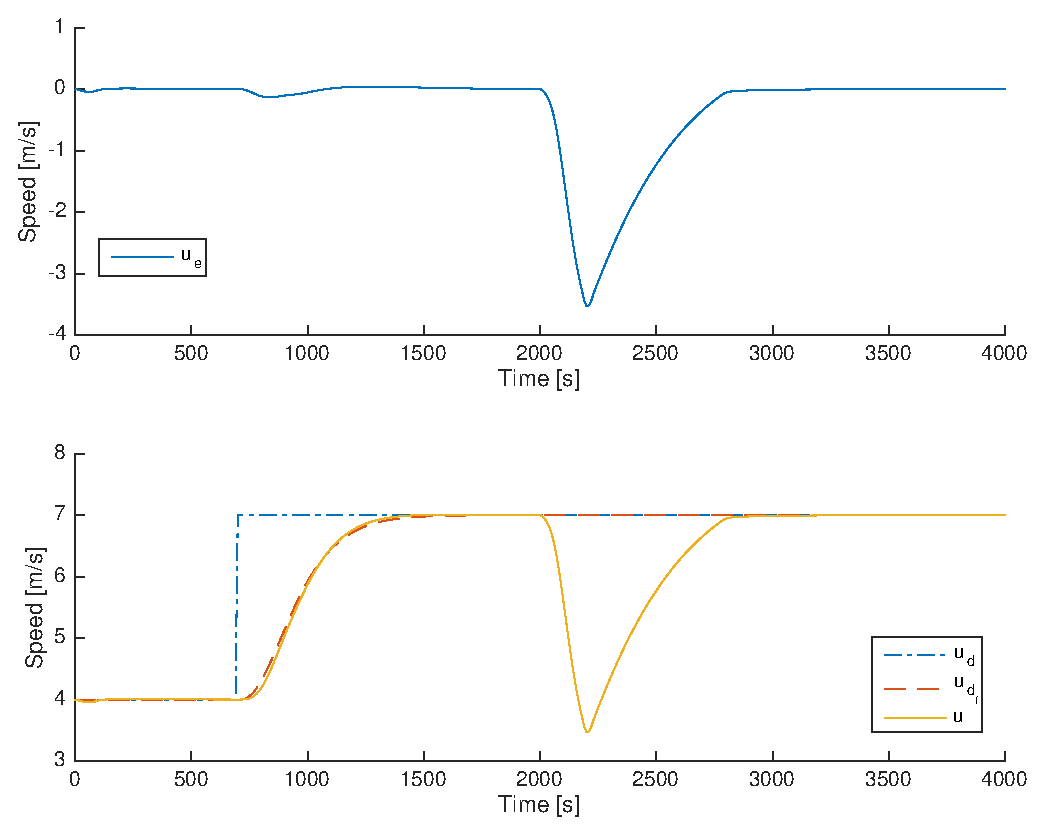
\includegraphics[width=0.9 \textwidth]{task1.8/Task1_8_sim}
    \caption{Speed step response}
    \label{fig:1.8-step}
\end{figure}